\section{Classification Methods}
To predict the publication conference, I formulated the supervised learning
framework to do classification. The conferences are treated as labels, and the
goal is to predict which conference a publication would belong to. Different
classifiers would have different view of this problem. I would introduce how to
use several most popular classifiers for this task.


\subsection{Scalable Smoothed Naive Bayes}
Naive Bayes is one of the most common basic classifiers with good performances.
Naive Bayes is suitable for text classification, like email spam detection
\cite{metsis2006spam}. Naive Bayes generally assumed the features are conditionally
independent over the classification labels. Therefore, with bayes rule, we could
derive:

\begin{equation*}
log P(y') = \sum_j log \frac{C (X_j=x_j \& Y=y')}{C (X=* \& Y=y')} +
log \frac{C (Y=y')}{C (Y=*)}
\end{equation*}

In general, we would add $\lambda$ smooth to avoid zero count case for Naive
Bayes. Besides, in most cases, we do not care the order of word features, which
means we would use bag of words model for Naive Bayes. With these assumptions,
we could derive:

\begin{equation*}
log P(y') = \sum_j log \frac{C(X=x_j \& Y=y')+\lambda}
{C(X=* \& Y=y') + \lambda \cdot \abs{X} } +
log \frac{C (Y=y')+\lambda}{C (Y=*)+\lambda \cdot \abs{Y} }
\end{equation*}

Naive Bayes is efficient for large scale dataset. We could use the stream and
sort pattern, which is also know as map-reduce, to make it scalable:

\begin{center}
\begin{minipage}{.75\linewidth}
\begin{algorithm}[H]
    \SetKwData{Left}{left}\SetKwData{This}{this}\SetKwData{Up}{up}
    \SetKwFunction{Union}{Union}\SetKwFunction{FindCompress}{FindCompress}
    \SetKwInOut{Input}{Input}\SetKwInOut{Output}{Output}

    \Input{Documents D with words X, and document labels Y}
    \Output{Trained Smoothed Scalabel Naive Bayes Classifier}
    \BlankLine
    \ForEach{publication with label y, and d words $x_1$, $x_2$, ...}{
        \BlankLine
        (a) Print $Y = ANY += 1$\;
        (b) Print $Y = y += 1$\;
        (c) \ForEach{word index j in 1,..d}{
                Print $Y = y \& X = x_j += 1$\;
            }
    }
    \BlankLine
    Sort the event-counter update message
    \BlankLine
    Scan and add the sorted meesage and get the final trained classifier
    \BlankLine
\caption{Scalable Smoothed Naive Bayes}
\end{algorithm}
\end{minipage}
\end{center}


\subsection{Decision Trees}
Systems that construct classifiers are one of the commonly used tools in machine
learning. Such systems take as input a collection of cases, each belonging to one
of a small number of classes and described by its values for a fixed set of
attributes, and output a classifier that can accurately predict the class to
which a new case belongs \cite{wu2008top}.

These algorithms are generally categorized as Decision Trees. Decision Trees
always achieve good performances in real-life applications. Complex decision
trees can be difficult to understand, for instance because information about one
class is usually distributed throughout the tree \cite{wu2008top}. Here we used
the C4.5 alogirithm which are implemented in Weka. C4.5 introduced an alternative
formalism consisting of a list of rules of the form “if A and B and C and ...
then class X”, where rules for each class are grouped together. A case
is classified by finding the first rule whose conditions are satisfied by the
case; if no rule is satisfied, the case is assigned to a default class
\cite{wu2008top}.


\subsection{SVM}
In today’s machine learning applications, support vector machines (SVM) are
considered a must-try. It offers one of the most robust and accurate methods
among all well-known algorithms. It has a sound theoretical foundation, requires
only a dozen examples for training, and is insensitive to the number of
dimensions. In addition, efficient methods for training SVM are also being
developed at a fast pace\cite{wu2008top}.

SVM are well introduced in Scholkopf and Smola's work \cite{scholkopf2002learning}.
Here we used the Weka SMO implementation for our task. The reason why SVM
insists on finding the maximum margin hyperplanes is that it offers the best
generalization ability. It allows not only the best classification performance
on the training data, but also leaves much room for the correct classification
of the future data \cite{wu2008top}. Besides, SVM has a good form and allows
kernelized methods which could transfer input data into a hyper space.


\subsection{Neural Networks}
Neural Networks are quite popular in recent days because of its impressively
good performances. With Neural Networks, we could both get better features and
better classifiers, although not well interpreted. While most remarkable
applications of Neural Networks are in computer vision filed, there are still
influential works used for text mining \cite{hochreiter1997long}
\cite{bengio2003neural}.

Here we just composed basic two layer neural networks since our training goal is
not very complex and the training data is not of very large scale.

\begin{figure}[!htbp]
    \centering
    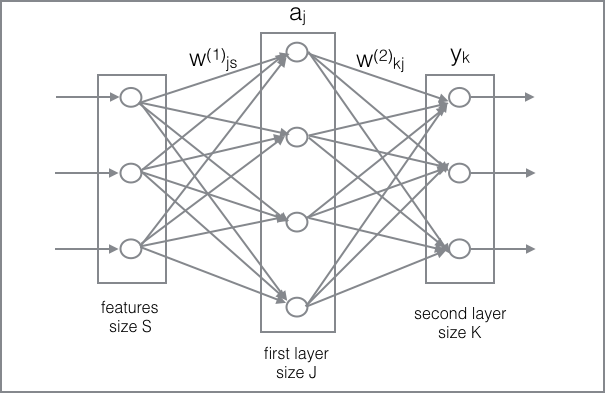
\includegraphics[width=8cm]{./pic/NN.png}
    \caption{Two Layer Neural Networks}
\end{figure}

The first layer was size J with j as index (j $>$ k).

\begin{equation}
a_{j} = \sigma (\sum_s w_{js}^{(1)} c_{s}), \qquad
\sigma (x) = \frac{1}{1 + e^{-x}}
\end{equation}

The size of second layer was K, with k as index:

\begin{equation}
y_k = \sum_j w_{kj}^{(2)} z_{j}, \qquad
\alpha_k = h(y_k)
\end{equation}

After we get $y_{k}$, we use softmax to get h for multi-label classification:

\begin{equation}
h(y_k) = \frac{e^{y_{k}}}{\sum_{k} e^{y_{k}}}
\end{equation}

The Neural Networks are implemented via mxnet, an open-source library on github.
Mxnet enables symbolic configuration, executor binding, and offers python interfaces,
which make the implementation easier.

